% ||||||||||||||| <<<<< COMPILIEREN MIT pdflatex --shell-escape Dima-Hadoop-Vortrag.tex >>>>>> ||||||||||||||||||||||||||

\documentclass{beamer}

% ++++++++++++++++++++++++++++++++++++++++++++++++++++++++++++++++++ 
% +++ Theme ++++++++++++++++++++++++++++++++++++++++++++++++++++++++
% ++++++++++++++++++++++++++++++++++++++++++++++++++++++++++++++++++ 
\usetheme{dima}
\logo{
\includegraphics[width=1cm]{dimalogo.pdf}}

% ++++++++++++++++++++++++++++++++++++++++++++++++++++++++++++++++++ 
% +++ Positionierung und Beschriftung von Bildern ++++++++++++++++++
% ++++++++++++++++++++++++++++++++++++++++++++++++++++++++++++++++++ 
% enable eps graphic files
\usepackage[cleanup={log,aux,dvi,ps,pdf}]{auto-pst-pdf}
% enable absolute positioning on frames
\usepackage[absolute,overlay]{textpos}
% adjust the TPHorizModule and TPHorizModule units to the displayed mm grid Anzahl der horizontalen und vertikalen Linien des Beamer Grids
\TPGrid{13}{10}
% beschriftungen
\usepackage{overpic}
% grid for positioning \setbeamertemplate{background}[grid][step=1cm]

\usepackage{etex}
% ++++++++++++++++++++++++++++++++++++++++++++++++++++++++++++++++++ 
% +++ Encoding +++++++++++++++++++++++++++++++++++++++++++++++++++++
% ++++++++++++++++++++++++++++++++++++++++++++++++++++++++++++++++++ 
% verwende Vektorschriften, falls vorhanden
\usepackage[T1]{fontenc}

% Encodierung der Quelldatei latin1 = ISO 8859-1 ansinew = Windows applemac = Apple-Mac utf8 = UTF-8-Encoding
\usepackage[utf8]{inputenc}


% ++++++++++++++++++++++++++++++++++++++++++++++++++++++++++++++++++ 
% +++ Schriften ++++++++++++++++++++++++++++++++++++++++++++++++++++
% ++++++++++++++++++++++++++++++++++++++++++++++++++++++++++++++++++ 
% verwendete Schriften Doku:
% http://www.ctan.org/tex-archive/macros/latex/required/psnfss/psnfss2e.pdf
\usepackage{charter}
\usepackage[scaled=.92]{helvet}
\usepackage{courier}

% besseres Schriftbild Doku: http://www.ctan.org/tex-archive/macros/latex/contrib/microtype/microtype.pdf
\usepackage{microtype}


%++++++++++++++++++++++++++++++++++++++++++++++++++++++++++++++++++
%+++ Bilder +++++++++++++++++++++++++++++++++++++++++++++++++++++++
%++++++++++++++++++++++++++++++++++++++++++++++++++++++++++++++++++
% Für Floatobjekte
\usepackage{float}
% \FloatBarrier - Ermöglicht das forcierte Setzen von ausstehenden Floats. section macht vor jede section eine barrier.
\usepackage[section]{placeins} 

% Paket um Grafiken einbetten zu können
\usepackage{graphicx}
\graphicspath{{images/}}
\usepackage{subfigure}

% Zeilenumbruch bei Bildbeschreibungen.
%\setcapindent{1em}


%++++++++++++++++++++++++++++++++++++++++++++++++++++++++++++++++++
%+++ Sprache ++++++++++++++++++++++++++++++++++++++++++++++++++++++
%++++++++++++++++++++++++++++++++++++++++++++++++++++++++++++++++++
% neue Deutsche Rechtschreibung: Trennregeln!
\usepackage[english]{babel}


%++++++++++++++++++++++++++++++++++++++++++++++++++++++++++++++++++
%+++ Literatur ++++++++++++++++++++++++++++++++++++++++++++++++++++
%++++++++++++++++++++++++++++++++++++++++++++++++++++++++++++++++++


\usepackage[
    backend=biber,
    url=true
]{biblatex}


\addbibresource{bib/references.bib}

%++++++++++++++++++++++++++++++++++++++++++++++++++++++++++++++++++
%+++ Verlinkung +++++++++++++++++++++++++++++++++++++++++++++++++++
%++++++++++++++++++++++++++++++++++++++++++++++++++++++++++++++++++
% Doku: http://www.ctan.org/tex-archive/macros/latex/contrib/hyperref/hyperref.pdf
%\usepackage[%
%pdfauthor={Erik Nijkamp and Alexander Alexandrov and Jan Marc Hoffmann},
%colorlinks, % verwende farbige Links
%linkcolor=blue, % Linkfarbe ist blau
%bookmarks, % erstelle Bookmarks der Links
%bookmarksopenlevel=1, % nur bis level 1 öffnen
%bookmarksopen, % Bookmarks werden beim öffnen des Dokumentes ebenfalls geöffnet
%urlcolor=blue, % Hyperlinks sind blau 
%citecolor=blue, % Cite Links sind blau
%bookmarksnumbered, % Bookmarks sind nummeriert
%final % Endversion 
%]{hyperref}

% fokusiert captions korrekt
%\usepackage[all]{hypcap}

\usepackage{listings}
% Listings Konfiguration
\lstset{language=Java, commentstyle=\color[RGB]{63,127,95}\ttfamily,
  keywordstyle=\color[RGB]{127,0,85}\bfseries,
  stringstyle=\color[RGB]{42,0,255}\ttfamily, showstringspaces=false,
  tabsize=2,
  % numbers=left,
  numberstyle=\tiny, numberblanklines=true, stepnumber=1,
  numbersep=5pt, xleftmargin=5pt,
  emphstyle=\color[RGB]{0,0,192}\texttt, breaklines=true,
  breakautoindent=true,
  % basicstyle=\tiny,
  extendedchars=true,
  % frame=shadowbox, rulesepcolor=\color{gray}
  %morekeywords={team,playedBy,as,when,after,before,base,within,replace,result,activate,deactivate}, %Erweiterung fuer Object Teams
  backgroundcolor=\color{white}, 
  framexleftmargin=2mm, 
  frame=shadowbox, 
  rulesepcolor=\color{lightgray}
}

% %%%%%%%%%%%%%%%%%%%%%%%%%%%%%%%%%%%%%%%%%%%%%%%%%%%%%%%% 
% Informationen zum Dokument
% %%%%%%%%%%%%%%%%%%%%%%%%%%%%%%%%%%%%%%%%%%%%%%%%%%%%%%%%

\author{\textcolor{gray}{Author:} Ward Schodts\\ \textcolor{gray}{Dozent:}
Pieter-Jan Kindermans}
\title{Concept drift}
%s\subtitle{lll}
\institute{Hot Topics in Machine Learning	 \\
Technische Universität Berlin \\[0.5cm]

\includegraphics[width=1.8cm]{tulogo}}
%\university{ss}
\date{\today}

%%%%%%%%%%%%%%%%%%%%%%%%%%%%%%%%%%%%%%%%%%%%%%%%%%%%%%%%%%%%%%%%
% Commands
%%%%%%%%%%%%%%%%%%%%%%%%%%%%%%%%%%%%%%%%%%%%%%%%%%%%%%%%%%%%%%%%

% Voor frames
\usepackage{mdframed}
% Voor kleuren
\usepackage{xcolor}

\definecolor{solarback}{HTML}{d9d9d9}
\definecolor{solarfront}{HTML}{000000}
\mdfdefinestyle{de}{linewidth=0pt,backgroundcolor=solarback,fontcolor=solarfront}
\newenvironment{de}[1]
{\begin{mdframed}[style=de]\begin{mydef}{\textbf{#1:}}\\} 
{\end{mydef}\end{mdframed}}
\newtheorem{mydef}{}

\usepackage{caption}
\captionsetup[figure]{labelformat=empty}

% %%%%%%%%%%%%%%%%%%%%%%%%%%%%%%%%%%%%%%%%%%%%%%%%%%%%%%%% 
% Dokument 
% %%%%%%%%%%%%%%%%%%%%%%%%%%%%%%%%%%%%%%%%%%%%%%%%%%%%%%%%%

\begin{document}

% --------------------------------------------------------
\begin{frame}
\maketitle
\end{frame}
%--------------------------------------------------------

%--------------------------------------------------------
\begin{frame}
\frametitle{Agenda}
\tableofcontents
\end{frame}
%--------------------------------------------------------

% %%%%%%%%%%%%%%%%%%%%%%%%%%%%%%%%%%%%%%%%%%%%%%%%%%%%%%%% 
% Folien 
% %%%%%%%%%%%%%%%%%%%%%%%%%%%%%%%%%%%%%%%%%%%%%%%%%%%%%%%%%

\section{Introduction}

% --------------------------------------------------------------------------------------------------------------

\begin{frame}
\frametitle{Introduction}

\begin{figure}
\centering

\includegraphics[width=\textwidth]{data}
\end{figure}

\end{frame}


\begin{frame}
\frametitle{Introduction}

\begin{figure}
\centering

\includegraphics[width=0.75\textwidth]{data}
\end{figure}

\LARGE Total volume of data generated: $>3$ zetabytes

\end{frame}


% --------------------------------------------------------------------------------------------------------------

% --------------------------------------------------------------------------------------------------------------
\begin{frame}
\frametitle{Introduction}
\begin{itemize}
\item<1-5> Traditionally all this data is processed in an \textit{offline} mode
\item<2-4> Due to the big amount of data
\item<2-4> And the expansion in forms as streams
\item<3-4> We can't do this anymore if we want to keep up.


\end{itemize}

\only<4>{\Large $\rightarrow$ We need an online solution}

\end{frame}
% --------------------------------------------------------------------------------------------------------------

\section{Adaptive Learning Algorithms}

% --------------------------------------------------------------------------------------------------------------
\begin{frame}
\frametitle{Adaptive Learning Algorithms}

\begin{de}{Adaptive Learning Algorithm}
can be seen as advanced incremental learning
algorithms that are able to adapt to evolution of the data-generating process over time.
\end{de}

It needs to be able to:
\begin{enumerate}

\item detect concept drift (and adapt if needed) as soon as possible;

\item distinguish drifts from noise and be adaptive to changes, but robust to noise; and

\item operate in less than example arrival time and use not more than a fixed amount of
memory for any storage.
\end{enumerate}


\end{frame}
% --------------------------------------------------------------------------------------------------------------

\begin{frame}
\frametitle{Online Adaptive Learning Procedure}

\begin{figure}
	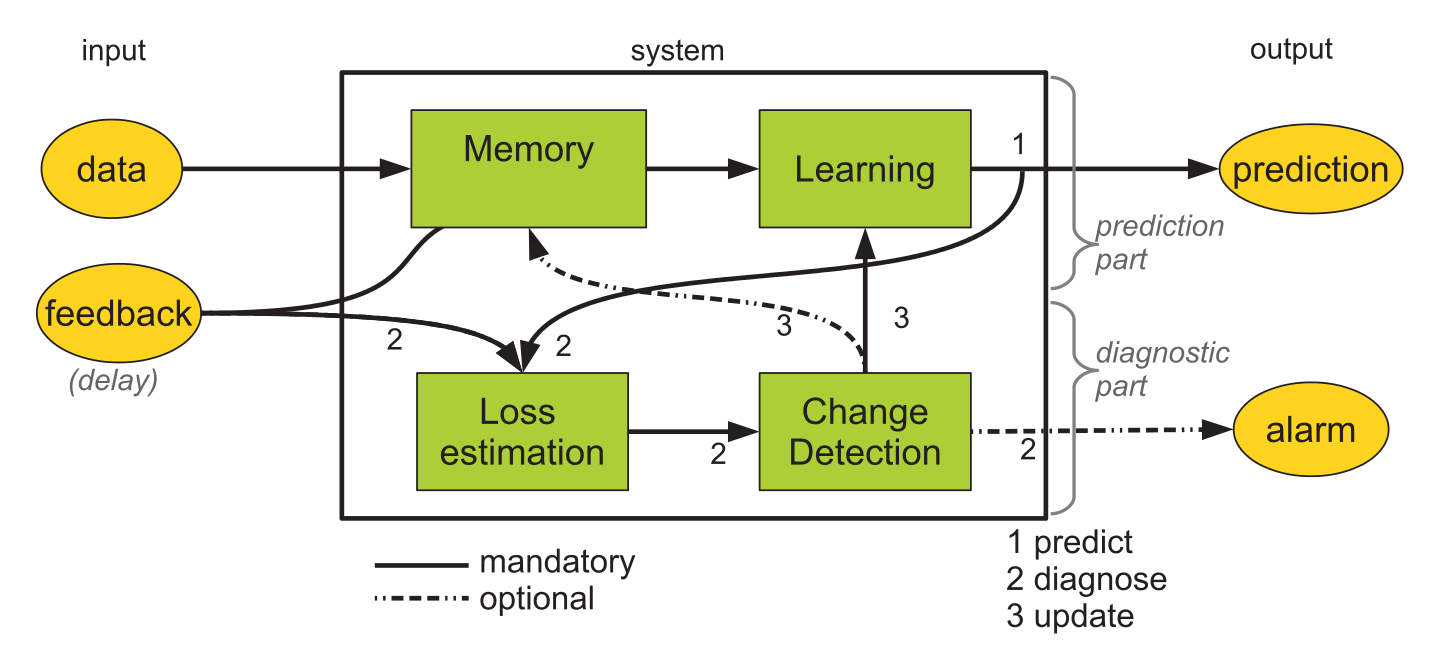
\includegraphics[width=0.75\textwidth]{modelala}
\end{figure}

\begin{enumerate}
	\item \textit{Predict.} When new example $X_t$ arrives, a prediction $\hat{y_t}$ is made using the curren model $L_t$.
	\item<2-3> \textit{Diagnose.} After some time, the true label $y_t$ and can estimate the loss as $f(\hat{y_t}, y_t)$.
	\item<3> \textit{Update.} We can use the example $(X_t,y_t)$ for the model update to obtain $L_{t+1}$.
\end{enumerate}

\end{frame}


% --------------------------------------------------------------------------------------------------------------
\begin{frame}[allowframebreaks]
\frametitle{Concept drift}
\begin{de}{Concept drift}
Formally, concept drift between time point $t_0$ and time point $t_1$ can be defined as:
$$\exists X:p_{t_0}(X,y) \neq p_{t_1}(X,y)$$

where $p_{t_0}$ denotes the joint distribution at time $t_0$ between the set of input variables X and the target variable y.
\end{de}


%Changes in data:

%\begin{itemize}
%\item prior probablities of classes $p(y)$ may change.
%\item class conditional probabilites $p(X|y)$ may change
%\item as a result the posterior probablities of classes $p(y|X)$ may change %(afftects the prediciton).
%\end{itemize}

\framebreak
$$\exists X:p_{t_0}(X,y) \neq p_{t_1}(X,y)$$
\begin{de}{Real concept drift}
refers to changes in $p(y|X)$. Such changes can happen either with
or without change in $p(X)$. It's also called \textit{concept shift} or \textit{conditional change}.
\end{de}

\begin{de}{Virtual concept drift}
happens if the distribution of the incoming data chagnes (i.e., p(X) changes) without affecting $p(y|X)$.
\end{de}
\end{frame}
% --------------------------------------------------------------------------------------------------------------


% --------------------------------------------------------------------------------------------------------------
\begin{frame}
\frametitle{Example: real vs. virtual drift}
\begin{figure}
	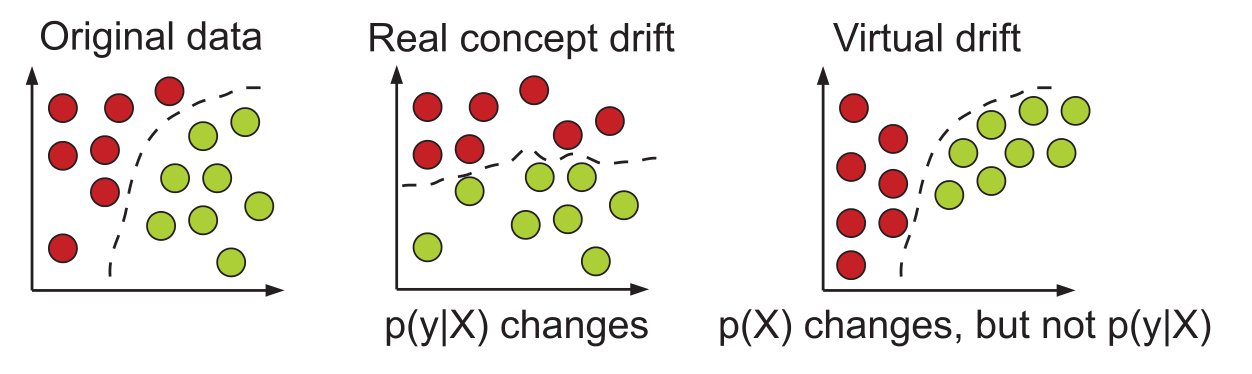
\includegraphics[width=\textwidth]{types}
\end{figure}
\textit{Circles} represent instances.\\
Different \textit{colors} represent different classes.

\end{frame}
% --------------------------------------------------------------------------------------------------------------

% --------------------------------------------------------------------------------------------------------------
\begin{frame}
\frametitle{A practical example: \# of people in a library}
\begin{figure}
	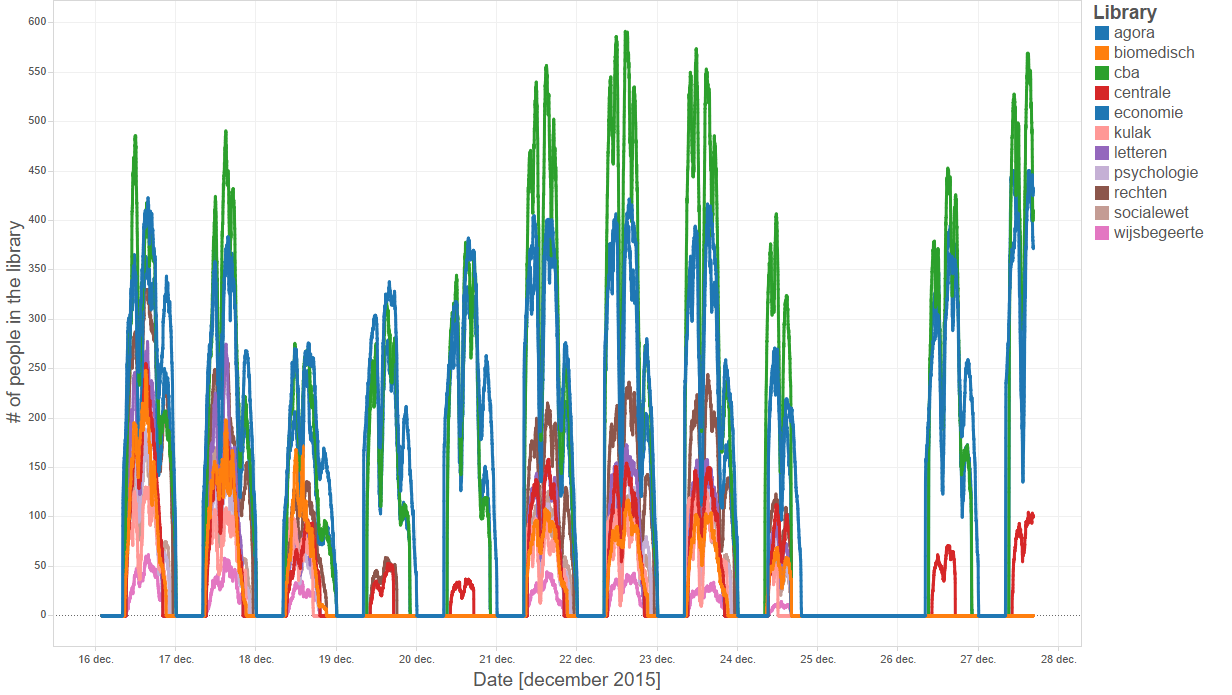
\includegraphics[width=\textwidth]{general_all}
	\caption	{\# of people in the KU Leuven libraries}
\end{figure}

\end{frame}

\begin{frame}
\frametitle{A practical example: \# of people in a library}
\begin{figure}
	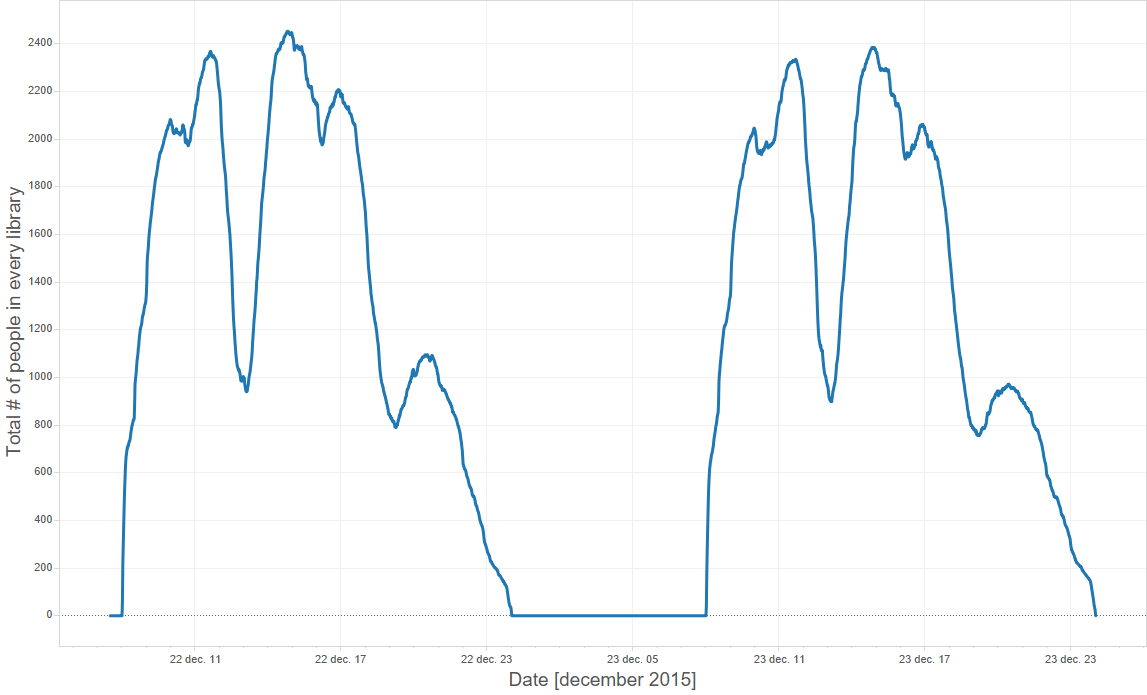
\includegraphics[width=0.75\textwidth]{total}
	\caption	{Sum of people in all KU Leuven libraries}
\end{figure}
\textbf{Task:} predict the total amount of people in all libraries\\
If same amount of people go to different libraries: \only<2>{$\rightarrow$ virtual drift}
\end{frame}
% --------------------------------------------------------------------------------------------------------------
\begin{frame}
\frametitle{A practical example: \# of people in a library}
\begin{figure}
	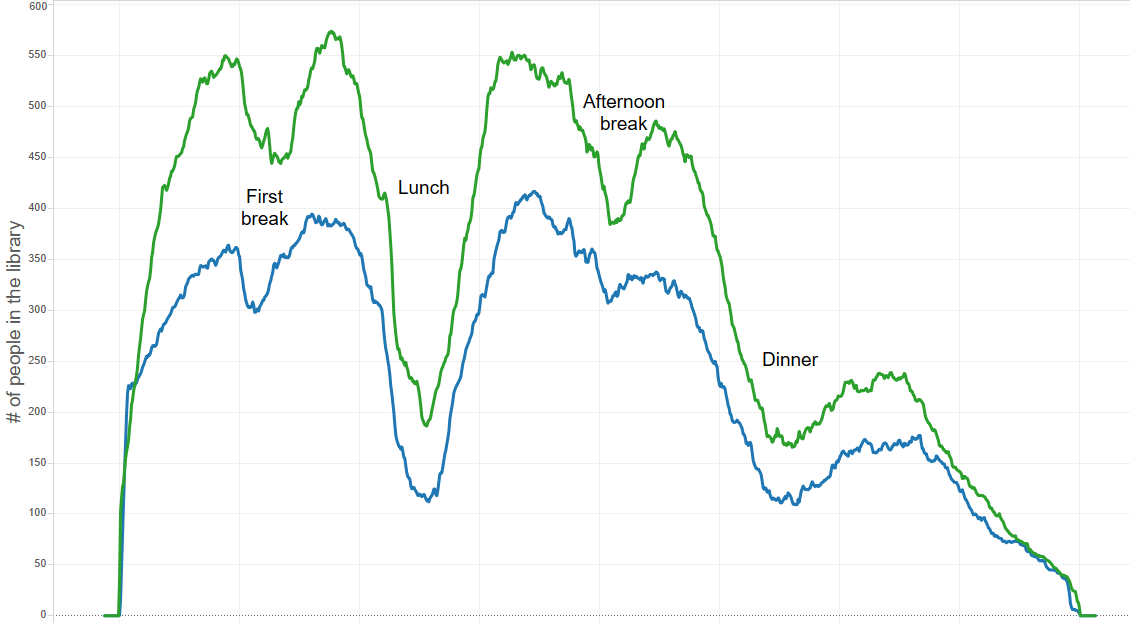
\includegraphics[width=0.75\textwidth]{comparison}
	\caption	{Sum of people in all KU Leuven libraries}
\end{figure}
\textbf{Task:} predict percentage of people in a specific library on a monday\\
If some people go to different libraries: \only<2>{$\rightarrow$ real drift}
\end{frame}

\begin{frame}
\frametitle{Changes in drift over time}

\begin{figure}[H]

	\begin{subfigure}[H]{0.2\textwidth}
		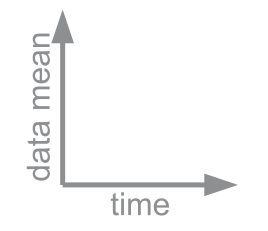
\includegraphics[width=\textwidth]{cot0}
	\end{subfigure}
	~
	\begin{subfigure}[H]{0.4\textwidth}
		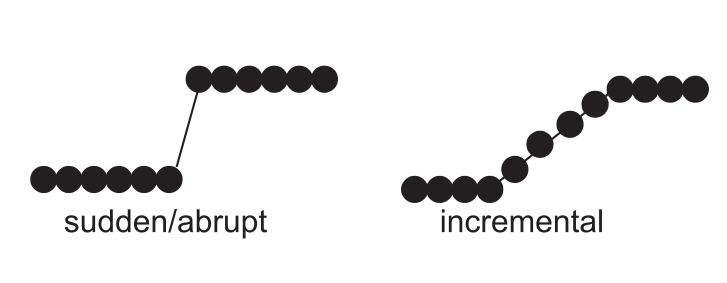
\includegraphics[width=\textwidth]{cot1}
	\end{subfigure}
	
	\only<2>{
	\begin{subfigure}[H]{0.2\textwidth}
		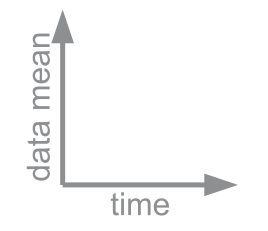
\includegraphics[width=\textwidth]{cot0}
	\end{subfigure}
	~
	\begin{subfigure}[H]{0.4\textwidth}
		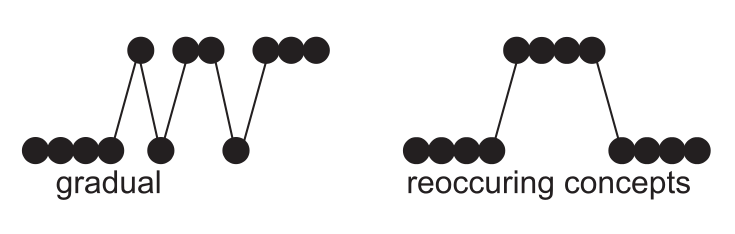
\includegraphics[width=\textwidth]{cot2}
	\end{subfigure}}
	
	\only<3>{
	\begin{subfigure}[H]{0.2\textwidth}
		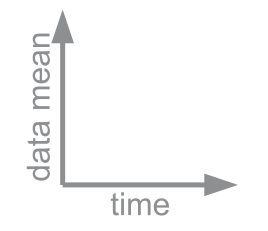
\includegraphics[width=\textwidth]{cot0}
	\end{subfigure}
	~
	\begin{subfigure}[H]{0.4\textwidth}
		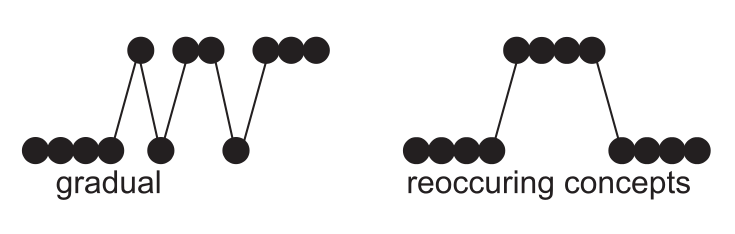
\includegraphics[width=\textwidth]{cot2}
	\end{subfigure}
	
	\begin{subfigure}[H]{0.2\textwidth}
		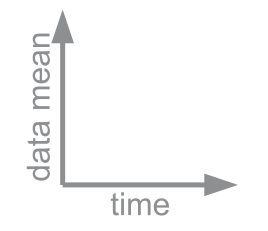
\includegraphics[width=\textwidth]{cot0}
	\end{subfigure}
	~
	\begin{subfigure}[H]{0.25\textwidth}
		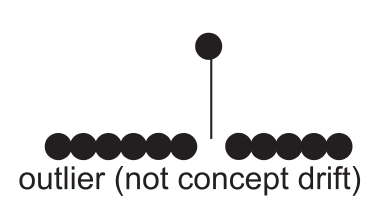
\includegraphics[width=\textwidth]{cot3}
	\end{subfigure}}
\end{figure}

\end{frame}


\begin{frame}
\frametitle{Changes in drift over time: library example}

\begin{figure}[H]
	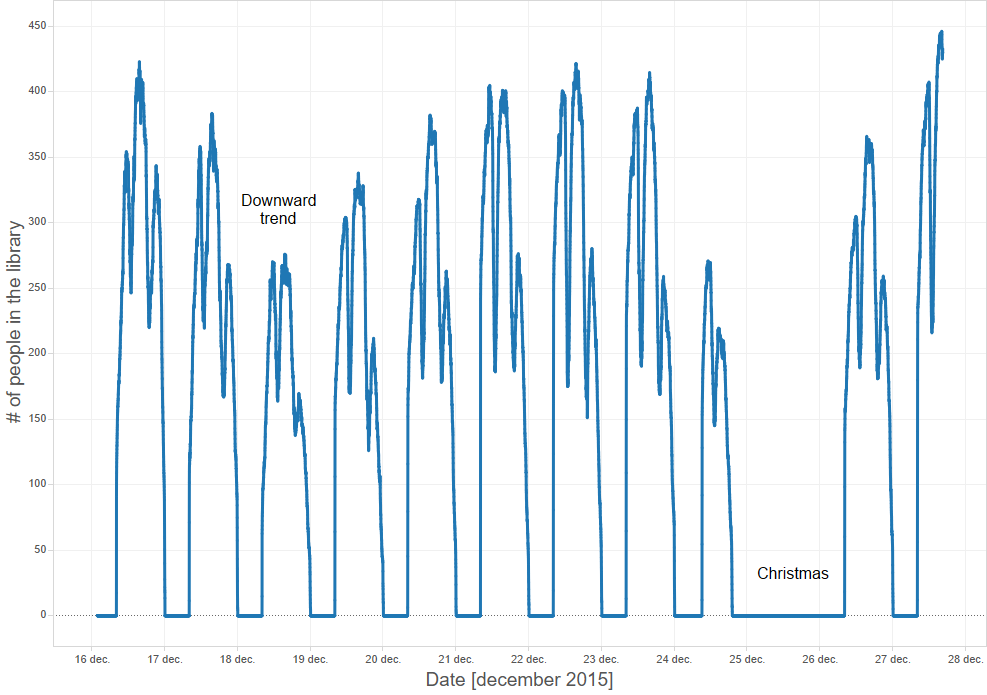
\includegraphics[width=\textwidth]{general}
\end{figure}
\end{frame}


\begin{frame}
\frametitle{Illustrative Applications}
\begin{itemize}
	
	\item Management and strategic planning
	\only<1>{
		\begin{figure}[H]
			\centering
			
\includegraphics[width=0.75\textwidth]{forecast}
		\end{figure}
	}
	
	\item Personal assistance and information
	\only<2>{
		\begin{figure}[H]
			\centering
			
\includegraphics[width=0.75\textwidth]{netflix}
		\end{figure}
	}
	
	\item Ubiquitous environment applications
	\only<3>{
		\begin{figure}[H]
			\centering
			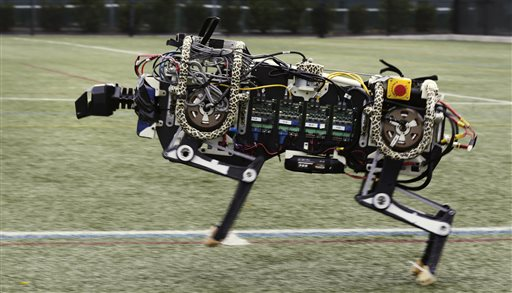
\includegraphics[width=0.75\textwidth]{cheetah}
		\end{figure}
	}
\end{itemize}
\end{frame}


\section{Methods for concept drift adaptation}
% ------------------------------------------------------------------------------
\begin{frame}
\frametitle{Agenda}
\tableofcontents[currentsection]
\end{frame}
% ------------------------------------------------------------------------------


% --------------------------------------------------------------------------------------------------------------
\begin{frame}
\frametitle{Methods for concept drift Adaptation}

\begin{figure}[H]
	\centering
	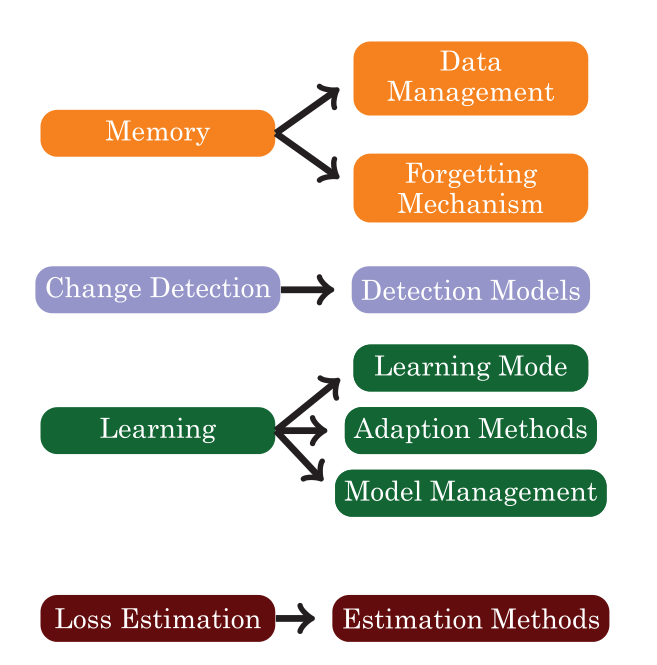
\includegraphics[scale=0.25]{mfcda/fourmodules}
\end{figure}

\end{frame}
% --------------------------------------------------------------------------------------------------------------

\subsection{Memory}

% ------------------------------------------------------------------------------
\begin{frame}
\frametitle{Agenda}
\tableofcontents[currentsubsection]
\end{frame}
% ------------------------------------------------------------------------------

% --------------------------------------------------------------------------------------------------------------
\begin{frame}
\frametitle{Memory in concept drift Adaptation}

\begin{figure}[H]
	\centering
	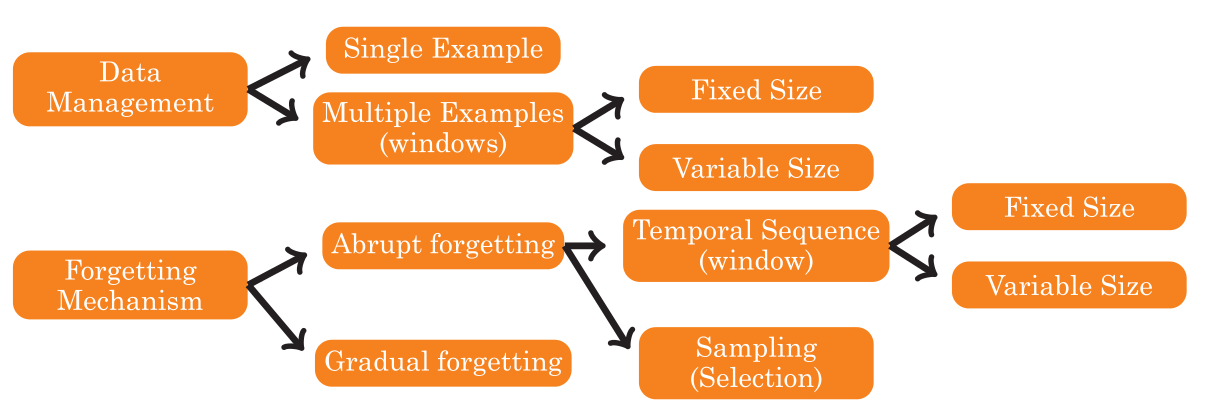
\includegraphics[width=\textwidth]{mfcda/memory}
\end{figure}

\end{frame}
% --------------------------------------------------------------------------------------------------------------








\subsection{Change Detection}

% ------------------------------------------------------------------------------
\begin{frame}
\frametitle{Agenda}
\tableofcontents[currentsubsection]
\end{frame}
% ------------------------------------------------------------------------------



\subsection{Learning}

% ------------------------------------------------------------------------------
\begin{frame}
\frametitle{Agenda}
\tableofcontents[currentsubsection]
\end{frame}
% ------------------------------------------------------------------------------

\begin{frame}



\end{frame}







\subsection{Loss Estimation}

% ------------------------------------------------------------------------------
\begin{frame}
\frametitle{Agenda}
\tableofcontents[currentsubsection]
\end{frame}
% ------------------------------------------------------------------------------


% --------------------------------------------------------------------------------------------------------------
\begin{frame}
\frametitle{Loss estimation in concept drift Adaptation}

\begin{figure}[H]
	\centering
	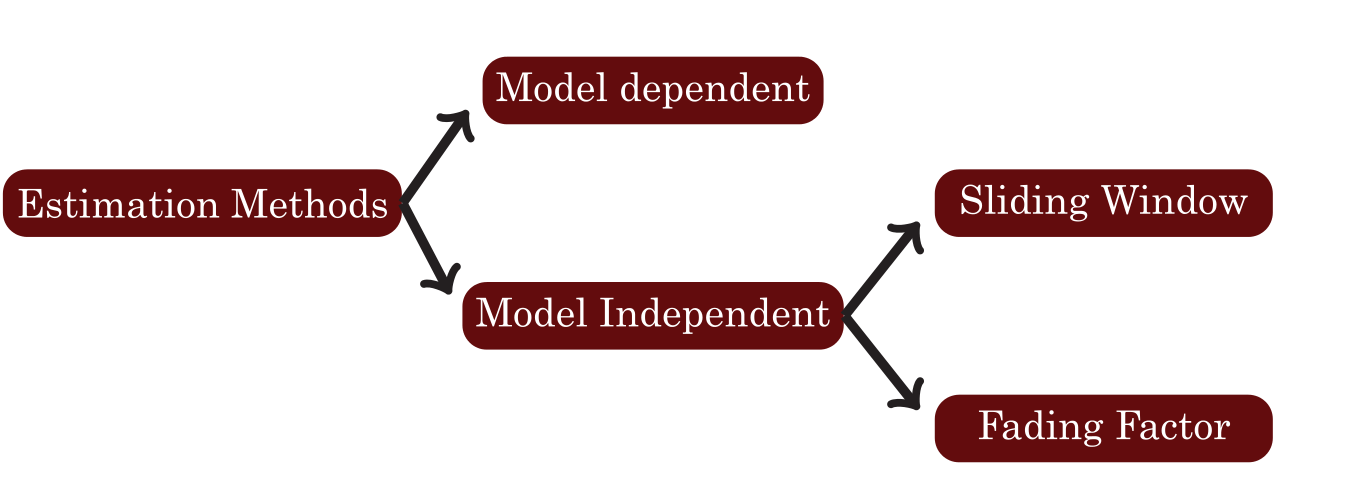
\includegraphics[scale=0.2]{mfcda/loss}
\end{figure}
\only<2>{
\begin{itemize}

\item \textbf{Model Dependent}
	\begin{itemize}
	\item Estimator needs to learn from the current model
	\item e.g. Klinkenbeg and Joachims \cite{klinkenberg} use it in SVM
	\end{itemize}

\end{itemize}
}

\only<3>{
\begin{itemize}

\item \textbf{Model Independent}
	\begin{itemize}
	\item Can be applied immediately
	\item \textbf{Sliding Window:} one small (quick) and one large (slower) together
	\item \textbf{Fading Factor:} a small FF detects change earlier
	\end{itemize}
\end{itemize}
}

\end{frame}




% --------------------------------------------------------------------------------------------------------------

\section{Evaluation}

% ------------------------------------------------------------------------------
\begin{frame}
\frametitle{Agenda}
\tableofcontents[currentsection]
\end{frame}
% ------------------------------------------------------------------------------

\begin{frame}
\frametitle{Evaluation}

For any machine-learning technique we want to evaluate we need:
\begin{enumerate}
\item Performance evaluation metrics chosen according to the goal of a learning task
\only<2>{\item A methodology allowing to compute the coresponding estimates (here in the streaming setting)}
\end{enumerate}

\end{frame}

\begin{frame}
\frametitle{Performance evaluation metrics}

\begin{itemize}
\item Traditional accuracy measures can be used:
	\only<1>{
	\begin{itemize}
	\item Precision and recall
	\item Weighted average
	\item Mean absolute sclaed errors
	\end{itemize}
	}
\item Use baseline approaches for some settings:
	\only<2>{
	\begin{figure}[H]
		\centering
		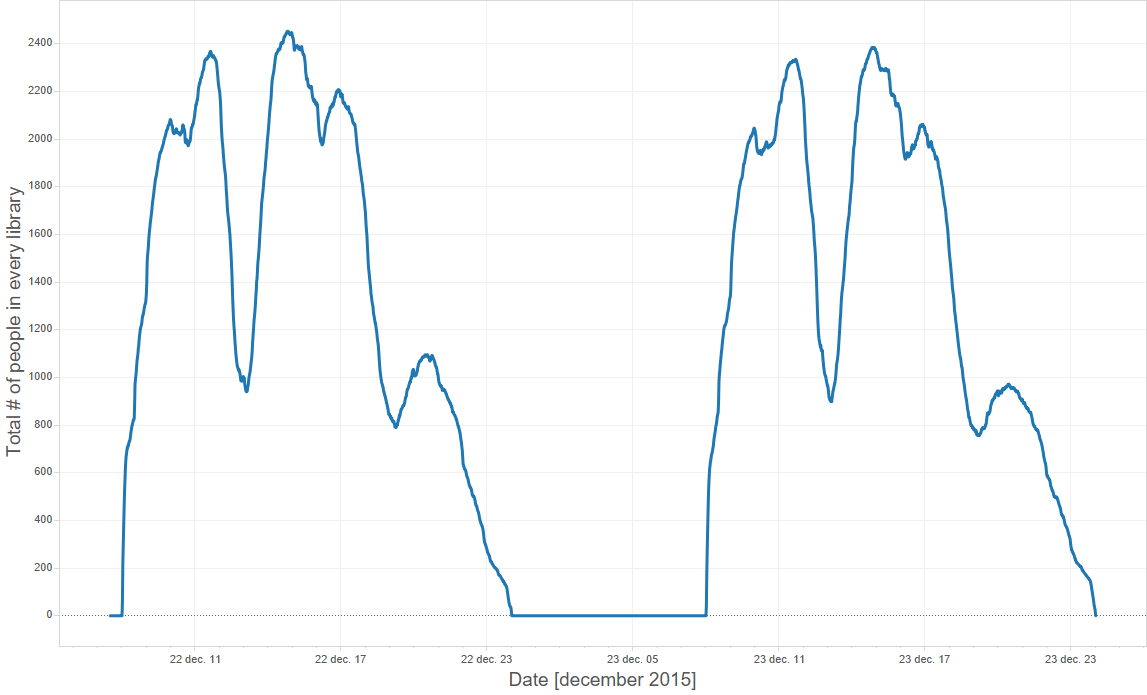
\includegraphics[scale=0.2]{total}
	\end{figure}}
\item Evaluating change detection methods:
	\only<3>{
	\begin{itemize}
	\item Probability of true change detection
	\item Probability of false alarms
	\item Delay of detection
	\end{itemize}
	}
\end{itemize}
\end{frame}

\begin{frame}
	\frametitle{Experimental Design}
	\begin{itemize}
		\item Cross-validation is not directly applicable
		\item Taking snapshots at different times
		\item Other techniques needed
	\end{itemize}

\end{frame}


\begin{frame}
	\frametitle{Evaluation of Time-Ordered Data}

	\begin{itemize}
		\item \textbf{Holdout:} keeping a subset
		\item \textbf{Interleaved Test-Then-Train:} check every instance first
		\item \textbf{Controlled Permutations:} run multiple test with permutated copies of the data
		\begin{itemize}
			\item (averaging accuracy might mask adaptation properties)
		\end{itemize}
	\end{itemize}

\end{frame}




\section{Conclusion}

% ------------------------------------------------------------------------------
\begin{frame}
\frametitle{Agenda}
\tableofcontents[currentsection]
\end{frame}
% ------------------------------------------------------------------------------


\begin{frame}
\frametitle{Conclusion}

\begin{itemize}
\item Concept drift is present in different application domains!
\item Concept drift is not only studied in machine learning and data mining or pattern recognition (e.g. processmining).
\item Next challenges:
	\begin{itemize}
	\item Scalability
	\item Robustness \& reliability
	\item Moving from \textit{black-box} adaptation to a more interpretable interpretation.
	\item Reducing dependence on timely and acurate feedback
	\end{itemize}
\end{itemize}
\end{frame}


%--------------------------------------------------------
\begin{frame}
\frametitle{Vielen Dank für Ihre Aufmerksamkeit}
\begin{center}
{\LARGE Fragen?}
\end{center}



\end{frame}

\begin{frame}[allowframebreaks]
		
        \frametitle{References}
        \nocite{*}
        \printbibliography

\end{frame}
%--------------------------------------------------------

\end{document}
